\subsection*{Problema 49}
\textbf{Enunciado:} Calcular la integral:
\begin{align*}
\int \dfrac{1}{x \sqrt{1 + x - x^2}} \, dx
\end{align*}

\textbf{Solución:} Para resolver la integral dada, utilizamos la sustitución recíproca sugerida. Sea:
\begin{align*}
u = \dfrac{1}{x} \implies x = \dfrac{1}{u}
\end{align*}

Calculamos el diferencial $dx$:
\begin{align*}
dx = -\dfrac{1}{u^2} \, du
\end{align*}

Sustituimos $x$ y $dx$ en la integral original:
\begin{align*}
\int \dfrac{1}{\left(\dfrac{1}{u}\right) \sqrt{1 + \dfrac{1}{u} - \left(\dfrac{1}{u}\right)^2}} \left(-\dfrac{1}{u^2} \, du\right)
\end{align*}

Simplificamos la expresión algebraica dentro del integrando:
\begin{align*}
= -\int \dfrac{\dfrac{1}{u^2}}{\left(\dfrac{1}{u}\right) \sqrt{1 + \dfrac{1}{u} - \dfrac{1}{u^2}}} \, du
\end{align*}

\begin{align*}
= -\int \dfrac{1}{u \sqrt{\dfrac{u^2 + u - 1}{u^2}}} \, du
\end{align*}

Como $u > 0$ en el dominio de interés, extraemos la raíz del denominador:
\begin{align*}
= -\int \dfrac{1}{u \left(\dfrac{\sqrt{u^2 + u - 1}}{u}\right)} \, du
\end{align*}

\begin{align*}
= -\int \dfrac{1}{\sqrt{u^2 + u - 1}} \, du
\end{align*}

Completamos el trinomio cuadrado perfecto bajo el radical:
\begin{align*}
u^2 + u - 1 &= \left(u^2 + u + \dfrac{1}{4}\right) - \dfrac{1}{4} - 1 \\
&= \left(u + \dfrac{1}{2}\right)^2 - \dfrac{5}{4}
\end{align*}

Sustituimos esto en la integral:
\begin{align*}
= -\int \dfrac{1}{\sqrt{\left(u + \dfrac{1}{2}\right)^2 - \left(\dfrac{\sqrt{5}}{2}\right)^2}} \, du
\end{align*}

Utilizamos la fórmula estándar de integración:
\begin{align*}
\int \dfrac{1}{\sqrt{z^2 - a^2}} \, dz = \ln\left|z + \sqrt{z^2 - a^2}\right| + C
\end{align*}

Aplicando la fórmula con $z = u + \dfrac{1}{2}$ y $a = \dfrac{\sqrt{5}}{2}$:
\begin{align*}
= -\ln\left|u + \dfrac{1}{2} + \sqrt{u^2 + u - 1}\right| + C
\end{align*}

Finalmente, regresamos a la variable original $x$ sustituyendo $u = \dfrac{1}{x}$:
\begin{align*}
= -\ln\left|\dfrac{1}{x} + \dfrac{1}{2} + \sqrt{\dfrac{1}{x^2} + \dfrac{1}{x} - 1}\right| + C
\end{align*}

\begin{figure}[H]
	\centering
	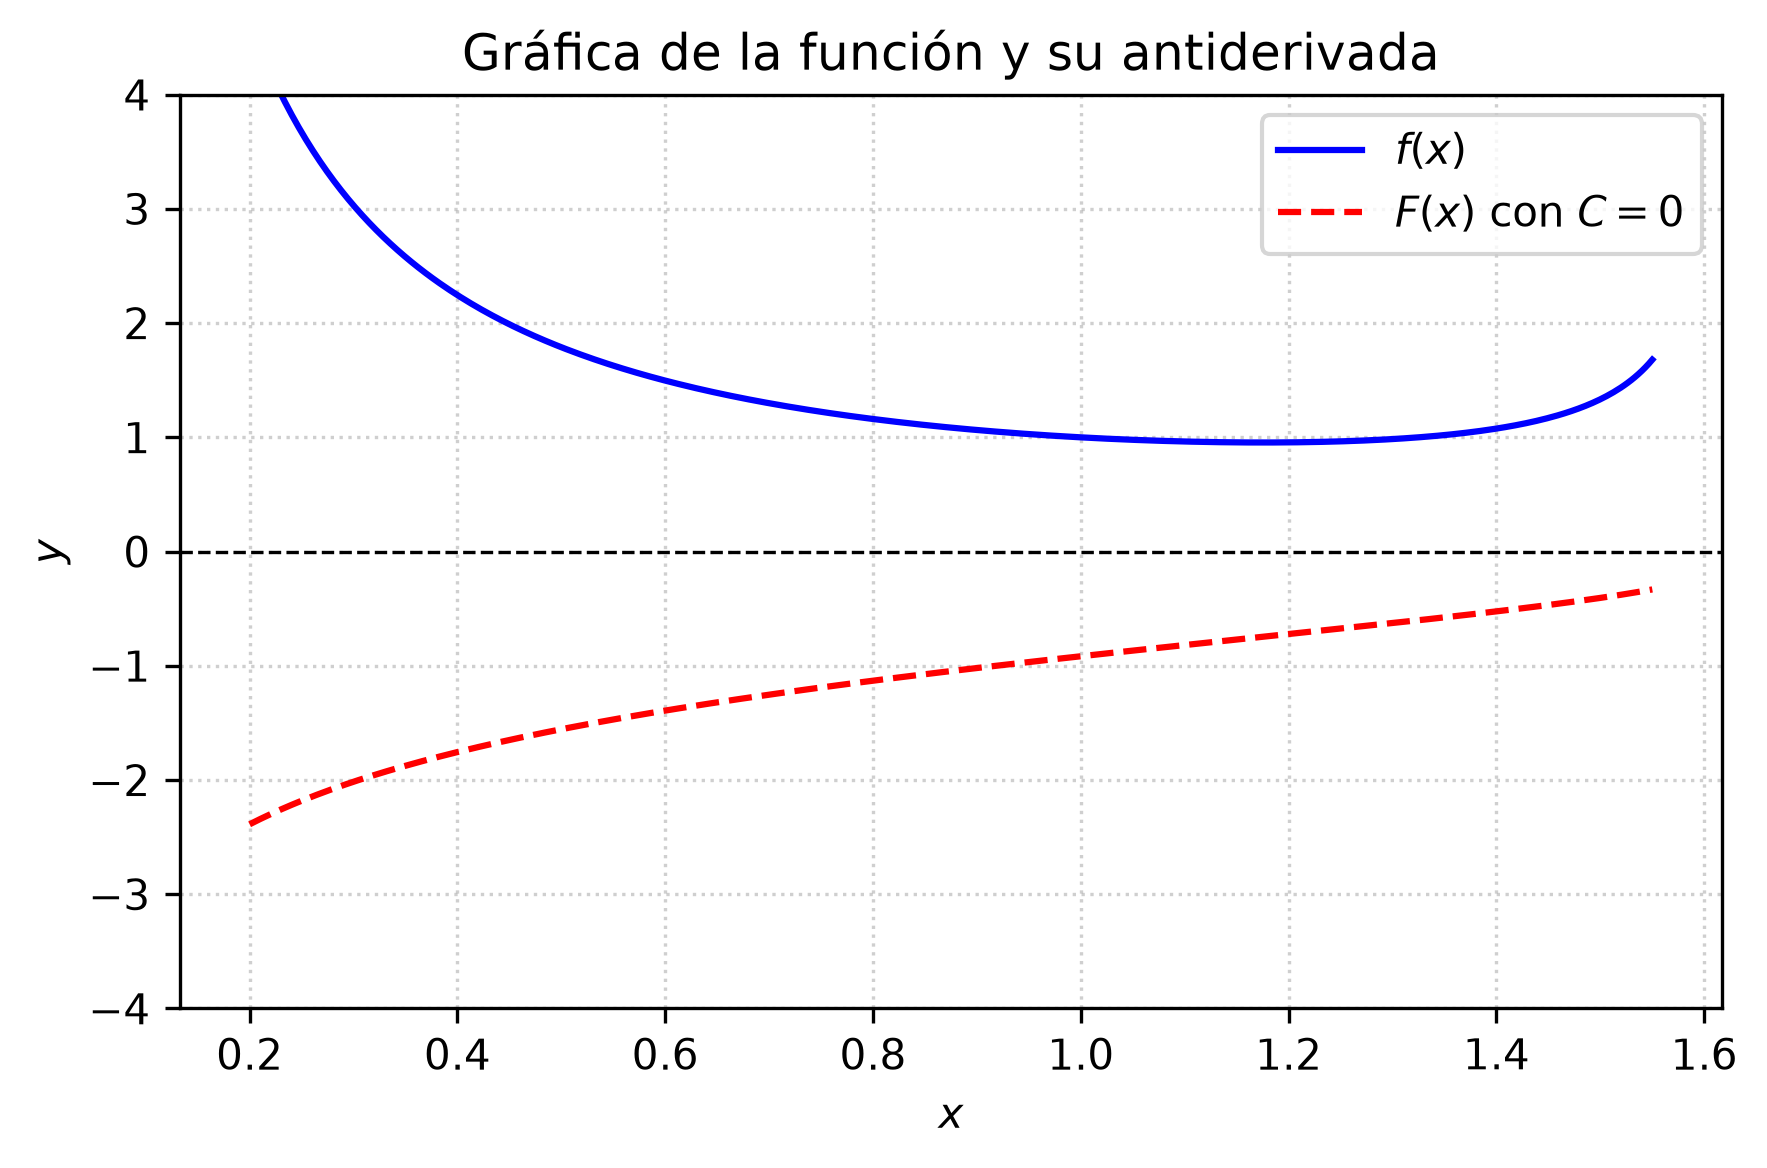
\includegraphics[width=\columnwidth]{semana_05/graficas/SEM05_P49_grafica.png}
	\caption{Representación gráfica de $f(x)$ y su antiderivada $F(x)$ evaluada para la constante de integración $C = 0$ (Problema 49).}
	\label{fig:problema49}
\end{figure}
